\chapter{稀疏复原:问题描述}\label{chap:srt01:problem}

本章的主要内容为稀疏信号复原中的优化问题。

从一个简单的不含噪线性观测情况开始,将之扩展为更为实际的含噪复原问题。问题的最终目的是寻找最稀疏解,也就是包含最少非零值的解,也称为$\ell_0$范数解,但由于其非凸组合本质,在计算上非常困难(确切地说是NP难问题),因此其求解必须借助近似方法。

稀疏复原中通常使用两种主要的近似方法,第一种是通过诸如贪婪搜索这样的近似方法来解决原始的NP难问题。第二种方法则是利用易于求解的凸松弛来代替棘手的原NP难问题。换言之,前者以近似方法解决精确问题,后者以精确方式解决近似问题。

考虑边界为$ \ell_0 $范数的$ \ell_p $范数族,并重点研究$ \ell_1 $范数,因为$ \ell_1 $范数是整个$ \ell_p $范数族中唯一能产生稀疏性并同时保持凸性的范数。

最后,从贝叶斯估计角度讨论稀疏信号复原和稀疏统计学习,引出最大后验概率参数估计(MAP)。与MAP方法相联系的是正则化优化,其中负对数似然和参数的先验分别对应损失函数和正则函数。

\section{不含噪稀疏复原}

继续使用之前的符号表示:$\mathit{x}=(x_1,x_2,\cdots,x_n)^T\in \mathbb{R}^N$为未观测的稀疏信号,$ y=(y_1,y_2,\cdots,y_m)^T\in \mathbb{R}^m $为观测值或观测向量,而$ A={a_{ij}}\in \mathbb{R}^{m\times n} $为设计矩阵。

从根据一组线性观测值复原无噪声信号这样最简单的问题开始,即求解线性方程组中的$ x $,
\begin{equation}\label{key}
Ax=y
\end{equation}
这里通常假设A是一个满秩矩阵,这样,对于任何$ y\in \mathbb{R}^m $,上述方程组有解。但需要注意的是,当未知变量的数量,即信号的维度,超过了观测值的数量,即$ m\leq n $时,上述方程组是欠定的,存在无数多个解。

为了复原信号$ x $,需要进一步对问题进行约束,或称为正则化。一般通过引入一个目标函数(或正则函数)$ R(x) $,以对信号额外的性质进行编码来实现,该目标函数或正则函数在取得期望解时具有较低值。因此,信号复原问题可以表述为以下约束优化问题:
\begin{equation}\label{key}
\min_{x\in \mathbb{R}^n}\: R(x)\quad s.t.\quad y=Ax
\end{equation}
例如,当希望得到的解具有稀疏性时,$ R(x) $就可以定义为非零元素的数量,或称为x的势,也称为$ \ell_0 $范数,表示为$ \Vert x \Vert_0 $。当腰注意,$ \ell_0 $范数并非严格意义上的范数,这一点会简要讨论。

一般的,特定$q$值的$ \ell_q $范数(表示为$ \Vert x \Vert_q $),经常用作正则函数,但更常见的是使用$ \ell_q $范数的$q$次幂$ \Vert x \Vert_q^q $作为正则函数。

现在详细研究$ \ell_q $范数的及其性质。当$ q\geq 1 $时,$ \ell_q $范数定义为:
\begin{equation}\label{key}
\Vert x \Vert_q = \left(\sum_{i=1}^{n}|x_i|^q\right)^{\frac{1}{q}}
\end{equation}


\begin{enumerate}
	\item 当$ q=2 $时,即为$ \ell_2 $范数,也称为欧几里得范数,是最常用的$ \ell_q $范数。
	\begin{equation}\label{key}
		\Vert x \Vert_2 = \sqrt{\sum_{i=1}^{n}|x_i|^2}
	\end{equation}
	\item 当$ q=1 $时,即为$ \ell_1 $范数。
	\begin{equation}\label{key}
		\Vert x \Vert_1 = \sum_{i=1}^{n}|x_i|
	\end{equation}
\end{enumerate}

现在我们回到向量的势及其与$ \ell_q $范数的关系。函数$ \Vert x \Vert_0 $被称为$ x $的$ \ell_0 $范数,定义为$ \Vert x \Vert_q^q $的极限,即当$ q\rightarrow 0 $时$ \ell_q $范数的第$ q $次幂:
\begin{equation}\label{key}
\Vert x \Vert_0 = \lim_{q\rightarrow 0}\Vert x \Vert_q^q = \lim_{q\rightarrow 0} \sum_{i=1}^{p}| x_i |^q = \sum_{i=1}^{p}\lim_{q\rightarrow 0} | x_i |^q
\end{equation}

而对于每一个$ x_i $,当$ q\rightarrow 0 $时,有$ |x_i\rightarrow I(x_i) $。$ x=0 $时,$ I(x) $值为0,否则为1.
因此可得,$\Vert x \Vert_0=\sum_{i=1}^{p}I(x_i)$,这给出了向量$ x $中非零元素的精确数量,也被称为势。利用势函数,现在可以将从不含噪线性观测值中复原稀疏信号的问题写成如下形式:
\begin{equation}\label{key}
(P_0):\quad  \min_{x} \Vert x \Vert_0 \quad s.t. \quad y =Ax
\end{equation}

上式中定义的$ (P_0) $问题是一个NP难问题,即目前没有算法能够在多项式时间内对其高效的求解。因此有必要借助近似方法。在恰当的条件下,最优或近似最优的解可以通过某近似方法来高效复原。
以下为两种常用的近似方法:
\begin{enumerate}
	\item {\heiti 利用基于启发式的搜索过程},如通过贪婪搜索以探寻问题$ (P_0) $的解空间。
	\begin{enumerate}
		\item 例如,可以从一个零向量开始,逐个增加非零坐标,在每一步中选择能够对目标函数值带来最佳该井的坐标。也叫贪婪坐标下降法。
		\item 一般地,这种启发式搜索方法并不能保证找到全局最优解。
		\item 但这种方法在实践中容易实现,计算效率非常高,并且常常能找到足够优的解。
	\end{enumerate}
    \item {\heiti 松弛方法},这种方法利用易处理的目标函数或约束来代替那些难以处理的目标函数
    \begin{enumerate}
    	\item 例如,凸松弛方法通过凸优化问题来近似非凸优化问题,也就是通过包含凸目标和凸约束的问题来近似非凸优化问题。
    	\item 这种凸优化问题通常是比较容易求解,存在很多优化方法来求解凸问题。
    	\item 显然,松弛的$ (P_0) $问题还必须保证解的稀疏性。
    \end{enumerate}
\end{enumerate}
\subsection{凸性的简单回顾}
几个概念:
\begin{enumerate}
	\item {\heiti 凸组合:} \\
	
	给定两个向量$ x_1\in \mathbb{R}^n $和量$ x_2\in \mathbb{R}^n $,以及一个标量 $ \alpha\in[0,1] $,向量$ x=\alpha x_1+(1-\alpha) x_2 $称为$ x_1 $和$ x_2 $的凸组合。
	\item {\heiti 凸集:}  \\
	
	如果集合$ S $中任何元素组成的凸组合任然属于该集合,那么该集合就称为凸集,即
	\[ \forall x_1,x_2 \in S,\quad\forall\alpha\in [0,1], \mbox{如果} x=\alpha x_1+(1-\alpha) x_2,\mbox{则} x\in S\]
	\item {\heiti 凸函数:} \\
	
	在一个向量空间上,定义于凸集合S上的函数$ f(x):S\rightarrow\mathbb{R} $称为凸函数的条件是
	\[ \forall x_1,x_2 \in S,\;\forall\alpha\in [0,1], \quad f(\alpha x_1+(1-\alpha) x_2)\leq \alpha f(x_1) + (1-\alpha)f(s_2) \]
	\begin{enumerate}
		\item 也就是说,连接凸函数曲线上两个点的线段总处于该函数曲线上方。
		\item 从几何角度来看,另一点解释方式是函数曲线上方的点组成的集合是凸的
		\item 如果上面的不等式是严格的,则该函数被称为严格凸函数
		\item 假设$ x_1 \neq x_2 $,且$ 0<\alpha<1 $,则凸函数的一个重要性质是其任意局部最小值也是全局最小值。而且严格凸函数具有唯一全局最小值。
	\end{enumerate}
\end{enumerate}

凸优化问题是凸函数在可行解的凸集上的最小化,其中可行解由约束来定义。由于凸目标函数的特性,凸问题比一般的优化问题易于求解。凸优化是优化相关文献中的一个传统研究领域,并且在过去若干年中已经有了许多高效的求解方法。

\subsection{问题$P_0$的松弛}
回到原问题$(P_0)$,即具有线性约束的势最小化。显然,约束$ y=Ax $产生了一个凸的可行集。事实上,给定两个满足这一约束的可行解$ x_1,x_2 $,两者的任意凸组合也是可行解。因为:
$$ A(\alpha x_1+(1-\alpha) x_2) = \alpha Ax_1 +(1-\alpha)Ax_2 = \alpha y+ (1-\alpha)y =y$$

因此,为了使问题$ (P_0) $松弛为一个凸问题,只需要用一个凸函数来代替目标函数$\Vert x \Vert_0  $,当然这里主要关注$ \ell_q $范数并将其作为$ \ell_0 $可能的松弛方法。

更精确的说,我们将研究$ \ell_q $范数的$ q $次幂,即函数$ \Vert x\Vert_q^q $,作为一般情况下的正则化函数$ R(x) $。对于一般情况下,当$ q\geq 1 $时,该函数为凸函数,当$ q<1 $时,其为非凸函数。


{\heiti 例如,$ \ell_2 $范数作为使用最广泛的$ \ell_q $范数,将其作为$ \ell_0 $范数的松弛也是自然而然的第一选择,可以得到问题$ (P_2) $}。
\begin{equation}\label{key}
(P_2):\quad  \min_{x} \Vert x \Vert_2^2 \quad s.t. \quad y =Ax
\end{equation}

函数$ \Vert x\Vert_2^2 $是严格凸的,并且具有唯一最小值。此外,问题$ (P_2) $具有解析闭合解。

{\heiti 求解问题$ (P_2) $可利用拉格朗日法。}

定义拉格朗日公式:
\begin{equation*}%\label{key}
\mathcal{L}(x)= \Vert x \Vert_2^2 + \lambda^{T}(y-Ax)
\end{equation*}

这里$\lambda$为一m维向量,其约束集合所对应的拉格朗日乘子。将上式两边对$ \lambda $求导可得::
\begin{equation*}\label{key}
\frac{\partial \mathcal{L}(x)}{\partial\lambda}= 2 x  +A^{T}\lambda 
\end{equation*}

令其等于0,即为上式的最优化条件。可得到唯一最优解如下:
\begin{equation*}\label{chap_srt01_x_l2opt}
x^*= -\frac{1}{2} A^T \lambda
\end{equation*}

因为$ x^* $必须满足约束条件$y= Ax$,将这个解带入约束条件,可得$ \lambda = -2(AA^T)^{-1}y $,即:
\begin{equation*}\label{key}
Ax* = -\frac{1}{2} A A^T \lambda = y  \Longrightarrow
\lambda = -2(AA^T)^{-1}y 
\end{equation*}

再将该结果带入式(\ref{chap_srt01_x_l2opt}),就可以得到常见的闭合形式的解析解:
\begin{equation*}\label{key}
x^* = -\frac{1}{2} A^T \lambda = A^{T}(AA^T)^{-1}b  = A^{+}b
\end{equation*}

当A的列数比行数多时,这个解被称为$ y=Ax $的伪逆解,这里要假定A是满秩的,即所有的行都是线性独立的。然而$\Vert x\Vert_2^2  $目标函数具有一个严重的缺陷,其最优解不是稀疏的,无法再稀疏信号复原中成为一个很好的近似方法。

\subsection{$\ell_q$-正则函数对接的稀疏性的影响}

{\heiti 如果你要要理解为何$ \ell_2 $范数无法得到解的稀疏性,而$ \ell_0 $范数却可以,要理解$ \ell_q $范数的凸性,以及导致稀疏的性质,则需要研究问题$ (P_q) $的几何结构。}
\begin{equation}\label{key}
(P_q):\quad  \min_{x} \Vert x \Vert_q^q \quad s.t. \quad y =Ax
\end{equation}

注意:{\heiti 	使得函数$ f(x) $具有相同值,即$ f(x)=const $的向量集合称为函数$ f(x) $的水平集。}
\begin{enumerate}
	\item 满足$ \Vert x\Vert_q^q \leq r^q $的向量集合称为半径为r的$\ell_q $球,其“表面”(集合边界)即为相应的水平集。
	\item 对于$ q\geq 1 $来说,以水平集为边界的$\ell_q $球是凸的,球上两点之间的直线仍在球内。
	\item 对于$ 0< q< 1 $来说,以水平集为边界的$\ell_q $球是非凸的,球上两点之间的直线并不总在球内。
\end{enumerate}

显然:{\heiti 	从几何视角来看,求解问题$ (P_q) $等价于以原点为中心“吹起”$ \ell_q $球,也就是说从0开始增加$ \ell_q $球半径,直到与超平面$ y=Ax $相交。相交点为最小$ \ell_q $范数向量。同时也是一个可行解,即为$ (P_q) $问题的最优解。}

注意,当$ q\leq 1 $时,$ \ell_q $球在坐标轴上有尖角,这些尖角与稀疏向量相对应,因为尖角的某坐标为0;但是当$ q>1 $时,$ \ell_q $球无此性质。因此,{\heiti 对于$ q\leq 1 $时,$ \ell_q $球可能与超平面$ Ax=y $在尖角处相交,从而产生稀疏解},而对于$ q>1 $,交点在实际中并不能在坐标轴上发生,解并不具有稀疏性。这是一个对$ \ell_q $范数性质直观的论证。

总的来说,我们既想要一个容易优化的函数来近似难于处理的$ \ell_0 $优化问题,又要产生稀疏解。在$\Vert x\Vert_q^q $ 函数族中,有:
\begin{enumerate}
	\item 仅当$ q\geq 1 $时,函数为凸函数。
	\item 仅当$ 0<q\leq 1 $时,可以产生稀疏解。
\end{enumerate}
\par 那么同时具有这两个性质的函数只有$\Vert x\Vert_1 $,即$ \ell_1 $范数。

同时具有稀疏性和凸性组合这一独一无二的性质,是$ \ell_1 $范数在现代稀疏信号复原领域广泛使用的原因。在不含噪情况下,难于处理的$ (P_0) $的$ \ell_1 $范数松弛可以表述为一下的问题$ (P_1) $,并成为理论与算法研究的主要焦点。
\begin{equation}\label{key}
(P_1):\quad  \min_{x} \Vert x \Vert_1 \quad s.t. \quad y =Ax
\end{equation}
\subsection{$\ell_1$范数最小化与线性规划的等价性}
{\heiti 问题$ (P_1) $可以转化为线性规划问题,后者作为优化问题已得到深入研究并具有高效的求解方法。}

事实上,引入新的非负变量$ u,v\in \mathbb{R}^n $,使得$ x =u-v $,其中,仅对$ x $的正值元素,有$ u_i $非0,其他元为0;对$ x $的负值元素,有$ v_i $非0,其他元为0。令$ z=[u^T,v^T]\in\mathbb{R}^{2n} $,可以得到:
\begin{equation*}\label{key}
\Vert x\Vert_1 = \sum_{i}^{2n}z_i
\end{equation*}

同时又有,$ Ax=A(u-v)=[A,-A]z $。那么问题$ (P_1) $等价于下面的线性规划$ (LP) $问题:
\begin{equation}\label{key}
\min_{z} \:\sum_{i}^{2n}\quad  s.t.\quad  y=[A,-A]z,\;\mbox{且}\:z\geq 0
\end{equation}

现在需要验证:{\heiti 对于一个最优解,上述关于$ u $与$ v $没有重叠支撑的假定是满足的,$ u $与$ v $分别对应$ x $中的征服元素。}

可利用反证法证明:{ 没看懂}
\begin{enumerate}
	\item 假设:对于某一$ j $,存在$ u_j $和$ v_j$皆非0.请示由于上述非负约束,有$ u_j>0,v_j>0 $。
	\item 不失一般性,假定$ u_j>v_j $,并用$ u^{'}_{j}=u_j-v_j $代替$ u_j $,$ v_j^{'}=0 $代替$ v_j $。很显然,非负约束仍然满足,同时线性约束$ y=[A,-A]z $也满足,既然$ A_j u_j -A_j v_j = A_j u^{j}_j - A_j v_j^{'} $,那么新解仍然是可行解。
	\item 然而,这样也将目标函数值降低了$ 2v_j $,与最初解的最优性相矛盾。
	\item 因此,可以说$ u $与$ v $没有重叠,即最初关于将$ x $分解为仅为正或仅为负的假设是成立的。
	\item {\heiti 那么问题$(P_1)$确实等价于上面的线性规划问题。}
\end{enumerate}




\section{含噪稀疏复原}
在实际应用中,如图像处理或统计数据建模,观测噪声是不可避免的。因此线性方程约束$Ax=y $必须被松弛,从而允许“理想的”观测$ AX $与其实际含噪版本之间存在离差。{\heiti 通常用不等式$ \Vert y-AX\Vert_2\leq \varepsilon $来代替原线性模型},表明实际观测向量$ y $与不含噪观测$ AX $之间的距离在欧式范数下不高于$ \varepsilon $。从概率角度来讲,如后面所讨论的,欧式范数来源于观测具有高斯噪声这个假设。其他噪声模型将产生更广泛类型的距离形式。
	
这样的松弛对于探究原始不含噪问题$ (P_0) $的近似解时有帮助的。而且当观测数量超过未知参数时,即$ A $的行数大于列数时,松弛时非常有必要的。在该情况下,线性方程组$ AX=y $可能误解,而这个问题是古典回归问题中经常碰到的。

含噪稀疏复原问题可被写成:
\begin{equation}\label{key}
(p_{0}^{\epsilon}):\qquad \min_{x}\Vert x\Vert_0\quad s.t.\quad\Vert y-Ax\Vert_2\leq \varepsilon
\end{equation}

对应的$ \ell_1 $范数松弛的含噪稀疏复原问题可以写成:
\begin{equation}\label{key}
(p_{1}^{\epsilon}):\qquad \min_{x}\Vert x\Vert_1\quad s.t.\quad\Vert y-Ax\Vert_2\leq \varepsilon
\end{equation}

上述约束也可修改为$ \ell_2 $范数平方的约束,即$ \Vert y-Ax\Vert_2^2<v $,其中$ v=\varepsilon^2 $,这时问题可以写作:
\begin{equation*}\label{key}
(p_{1}^{\epsilon}):\qquad \min_{x}\Vert x\Vert_1\quad s.t.\quad\Vert y-Ax\Vert_2^2\leq v
\end{equation*}

利用恰当的拉格朗日乘子$ \lambda $,可以将上述问题转化为一个无约束的最小化问题:
\begin{equation}\label{key}
(p_{1}^{\lambda}):\qquad \min_{x} \dfrac{1}{2}\Vert y-Ax\Vert_2^2 + \lambda \Vert x\Vert_1 \qquad
\end{equation}

或者,对于某些前档的参数$ t(\varepsilon) $,可简写为$ t $,同样的问题可写作:
\begin{equation}\label{formula:chapsrt01:p1t}
(p_{1}^{t}):\qquad \min_{x} \dfrac{1}{2}\Vert y-Ax\Vert_2^2 \quad s.t.\quad \Vert x\Vert_1 \leq t
\end{equation}

如前所输,{\heiti 上述$ \ell_1 $范数正则化问题,特别是$(p_{1}^{\lambda})$和$(p_{1}^{t})$这两种形式,在统计学文献中被称为LASSO,在信号处理领域被称为基追踪。}

注意,如不含噪复原问题累死,$ (p_{1}^{\lambda}) $问题可以转化为半二次规划问题(QP),从而通过标准的优化工具箱进行求解,即:
\begin{equation}\label{key}
\min_{x_{+},x_{-}\in \mathbb{R}^{n}_{+}} \dfrac{1}{2}\Vert y-Ax_{+}+A_{-}\Vert_2^2 + \lambda (1^{T}x_{+}+1^{T}x_{-})
\end{equation}
 

\subsection{两种特例情况下的LASSO问题的几何解释}

\begin{enumerate}
	\item  [(a)]  $ n\leq m $,低维情况,观测数量大于变量数量
	\item  [(b)]  $ n>m $,高维情况,此时观测数量小于变量数量。
\end{enumerate}

(a)  $ m \geq n $,低维情况


在这两种情况下,$ \ell_1 $范数约束为具有“尖锐边缘”的菱形区域,其中,尖锐边缘对应着稀疏可行解。而上式中二次函数的水平集具有不同的形状,依赖于变量数量$ n $,是否超过观测数量$ m $。

在低维情况下,当$ n\leq m $时,只要矩阵A是列满秩的,即其列为线性独立的,那么式\ref{formula:chapsrt01:p1t}中的二次目标函数具有唯一最小值解$ \hat{x} =(A^TA)^{-1}A^T y $。

验证过程如下:
\begin{equation*}\label{key}
f(x)       =         \Vert y-Ax \Vert_2^2 = (y-Ax)^{T}(y-Ax)    
\end{equation*}

令其倒数为0,可得:
\begin{equation*}\label{key}
\dfrac{\partial f(x)}{\partial x}  = -2A^T(y-Ax) =0
\end{equation*}

从而可得其唯一解$ \hat{x} =(A^TA)^{-1}A^T y $。由于上述目标函数的最小化等价于求解基本的普通最小二乘回归问题,因此该解被称为普通最小二乘解(OLS),即
$$   OLS:\qquad  \min_{x}  \Vert y-Ax \Vert^2_2$$

当A的行数大于列数时,OLS解也被称为$ y=AX $的伪逆解。需要注意的是,即使线性方程组$ y =Ax $的解不存在时,伪逆解也是存在的。

目标函数$ \Vert y-Ax \Vert^2_2 =const $ 的水平集从最小值处的奇点$ \hat{x} $开始,对于较大的函数值,该水平集对应椭圆。

(b) $m<n $,高维情况

当$ m<n $时,A为行满秩矩阵,线性系统$ y=Ax $总是存在一个解,如问题$ P_{2} $的最小$ \ell_2 $范数解$\hat{x}=A^T (AA^T)^{-1}y $,即当列数大于行数的情况下$ y=Ax $的伪逆。

而且,存在无穷多个具有形式为$ \hat{x} +z $的解,其中$ z\in N(A) $,$ N(A) $为A的零空间,即空间中所有点集均使得$ Az=0 $,因此$ A(\hat{x}+z)=A\hat{x} =y$。所有这些解形成了一个超平面$ y=Ax $,与目标函数最小值的水平集相对应,即$ \Vert y-Ax\Vert_2^2 =0$。另一水平集$\Vert y-Ax\Vert_2^2 =const$与平行于$ Ax=y $的两个超平面相对应,这两个超平面与$ Ax=y $距离相等。


令$ t_0 =\min_{z\in N(A)} \Vert \hat{x}+z\Vert_1 $为线性系统$ y=Ax $的解({\color{red} 或$ m\geq n $情况下的单一解})达到的最小$ \ell_1 $范数。假定在式(\ref{formula:chapsrt01:p1t})中有$ t<t_0 $,{\color{red} 否则$ \ell_1 $范数约束是无意义的,即$ LASSO $问题变成无约束的普通最小二乘问题。}
那么,最小二乘解位于可行区域之外,式(\ref{formula:chapsrt01:p1t})的任意解$ x^* $必须为该区域的边界,即目标函数的水平集首先与可行区域相交,这意味着$ \Vert x\Vert_1 =t$。注意到菱形的可行区域$ \Vert x\Vert_1 <t $倾向于在菱形区域的最高点与二次函数相交,这在二维情况下很容易看到,在多维情况下也是如此,与稀疏解相对应。这个例子论证了对$ \ell_1 $范数约束强化稀疏性背后的直观理解,与不含噪声稀疏复原问题相似。


上面讨论的$ LASSO $问题的解现在可以总结如下:
\begin{theorem}[Osborne et al., 2000b]\quad\par
\begin{enumerate}
	\item 如果$ m\geq n$(样本数量比未知参数多),那么式\ref{formula:chapsrt01:p1t}中的$ LASSO$ 问题具有唯一解$ x^*$,且$ \Vert x^*\Vert_1 =t $。
	\item 如果$ m<n $(样本数量比未知参数少),那么$ LASSO $问题的解存在,且对于任意解有$ \Vert x^*\Vert_1 =t $。
	\item 如果$ x_1^* $和$ x_2^* $均为$ LASSO $问题的解,那么他们的凸组合$\alpha x_1^* +(1-\alpha)x_2^* $也为其解,其中$ 0\leq x\leq 1 $。
\end{enumerate}
\end{theorem}

\begin{lemma}[最优性条件]
向量$ \hat{x}\in\mathbb{R}^n $为$ LASSO $问题$ (P_1^{\lambda}) $的解,当且仅当下面的条件对$ i\in \{1,2,\cdots,n\} $均满足:
\[ \alpha^T_i(y-A\hat{x}) = \alpha sgn(\hat{x}_i)\qquad \mbox{若}\hat{x}_i\neq 0\]
\[ |\alpha^T_i(y-A\hat{x})|\leq \lambda \qquad\qquad \mbox{若}\hat{x}_i= 0 \]
其中$ \alpha_i $为矩阵A的第i列。
\end{lemma}


\section{稀疏复原的统计学视角}

在统计学习问题中,设计矩阵A的列与随机变量$ A_j $相对应,称为预测因子;设计矩阵A的
行与样本相对应,即与预测变量的观测相对应,该观测常家丁为独立同分布的。同时,$ y $
的元素与另一随机变量$ Y $的观测相对应,称为相应变量。目标是在给定预测因子的情况下,
通过学习过程得到能够预测相应的统计模型。

现在定义一个一般的统计学习框架。令$ Z=(A,y) $表示观测数据,即包含n个预测因子与相应
响应的m个样本集合,$ M(x) $表示含有参数$ x $的模型。

标准的模型选择方法假定了一个损失函数$ L(Z,x) $,该损失函数描述了观测数据与模型得到
的近似值之间的离差,如线性模型估计值$ \hat{y}=Ax $与实际观测$ y $之间的平方和损失。
模型选择通常看成是关于x的损失函数的最小化问题,目的是为了找出与数据最佳拟合的模型。

然而,当参数数量n大于样本数量m时,这样的方法会产生对数据的过拟合,即通过学习得到的
参数可以很好的表示训练数据,但是不能适用于测试数据。测试数据可能是来自于同一数据分
布但未使用的数据。因为统计学习最终的目的是得到模型的泛化精度,所以可以在优化问题上
增加一个额外的正则化约束,在搜索最小损失解时,通过限制参数空间来防止产生过拟合现象。

令$ R(x) $表示正则函数,那么模型选择问题通常可以表述为:
\begin{equation}\label{key}
\min_{x}\:  L(Z,x)\quad s.t.\quad R(x)\leq t
\end{equation}
也可以写作等价的形式,即:
\begin{equation}\label{key}
\min_{x}\: R(x) \quad  s.t.\quad L(Z,x)\leq \epsilon
\end{equation}
或者,使用一个合适的拉格朗日乘子$\lambda $,有:
\begin{equation}\label{key}
\min_{x}\:  L(Z,x)+\lambda R(x)
\end{equation}
其中,$ \epsilon $和$ \lambda $由t唯一确定,反之亦然。

{\heiti 下面,讨论损失函数和正则函数的概率解释。}

假定模型$ M(x) $描述了数据的概率分布$ P(Z|x) $,其中$ x $为该分布的参数。同时,根据贝
叶斯方法,假定参数的先验分布为$ P(x|\lambda) $,超参数$ \lambda $暂时假定为固定不变的。
那么,模型学习问题就可以转化为MAP参数估计问题,即寻找使得联合概率$ P(Z,x)=P(Z|x)P(x|\lambda) $
最大化。,或者说最小化负对数似然的参数$ x $值,即:
\begin{equation}\label{key}
\min_{x} -log\left [P(Z|x)P(x|\lambda)\right ]
\end{equation}
上式也可以写作:
\begin{equation}\label{key}
\min_{x} -\log P(Z|x) - \log P(x|\lambda)
\end{equation}
注意,学习问题的$ MAP $表述产生了上述正则损失最小化问题,损失函数$ L(Z,x)=-\log P(Z|x) $
的值越小,模型的似然越高,即对数据的拟合度越好。正则函数$ R(x,\lambda)=-\log P(x|\lambda) $
由模型参数的先验确定。

从数据中学习统计模型的MAP方法产生了广泛的问题表述。例如,含噪稀疏复原问题$ (P_1) $,即
$ \ell_1$正则平方和损失最小化,也成为稀疏线性回归,可以看做$ MAP $方法中具有线性高斯观
测与参数的拉普拉斯先验情况下的特例。


换言之,假定y的元素为独立同分布的随机变量,服从高斯分布,即
\begin{equation}\label{key}
N_{\mu,\sigma}(z)=\dfrac{1}{\sqrt{2\pi }\sigma}e^{-\frac{1}{2}(z-\mu)^2}
\end{equation}

当标准差$\sigma =1 $且均值$ \mu =\alpha_i x$($\alpha_i$为矩阵$ A $的第$ i $行)时。
\[  P(y_i|\alpha_i x)= \dfrac{1}{\sqrt{2\pi}}e^{-\frac{1}{2}(y_i-\alpha_i)^2}   \]

假定上述模型的参数$ x $固定,那么数据$ Z=(A,y) $的似然比为$ P(A,y|x)=P(y|Ax)P(A) $。
因此,负对数似然损失函数可以写作:
\begin{equation}\label{key}
\begin{split}
L(y,A,x) &= -\log P(y|Ax) - \log P(A) \\
         &= -\log \prod_{i=1}^{m}P(y_i|\alpha_i x) -\log P(A)\\
         &= \dfrac{1}{2}\sum_{i=1}^{m}(y_i-\alpha_i x)^2 +const
\end{split}
\end{equation}

其中$const=\log \sqrt{2\pi}-\log P(A)$并不依赖于$ x $,因此可以从上式中的目标函
数中省略。由y的线性高斯假设可以到处平方和损失函数,即:
\begin{equation*}\label{key}
L(y,A,x)  = \dfrac{1}{2}\sum_{i=1}^{m}(y_i-\alpha_i x)^2 = \dfrac{1}{2}\Vert y-Ax\Vert_2^2
\end{equation*}


\subsection{参数$ x_i $服从参数为$ \lambda $拉普拉斯先验}

下面假设参数$ x_i $服从参数为$ \lambda $拉普拉斯先验,其中$ i=1,\cdots,n $为独立
同分布随机变量,即:
\begin{equation}\label{key}
p(z) = \dfrac{\lambda}{2}e^{-\lambda|z|}
\end{equation}

下图显示了当$ \lambda $取不同值时的拉普拉斯分布的例子。注意当$ \lambda $增加时,
接近于0的值会被赋予更高的概率权重。
\begin{figure}
	\centering
	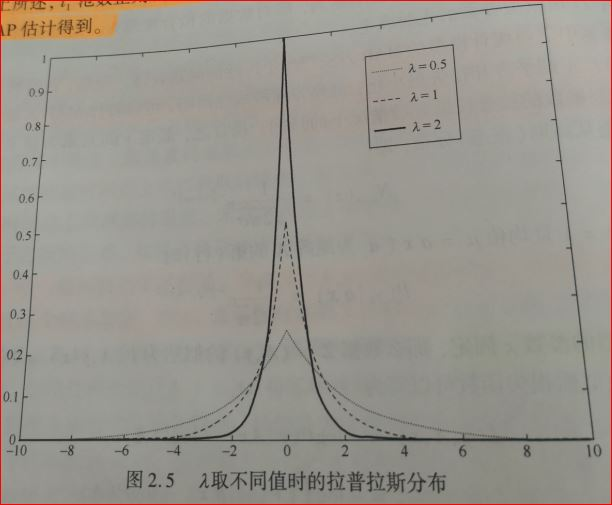
\includegraphics[width=0.7\linewidth]{Img/chap_srt01_problem/lap_lambda}
	\caption{$ \lambda $取不同值时的拉普拉斯分布}
	\label{fig:laplambda}
\end{figure}


当参数具有拉普拉斯先验时,正则函数可以写成
\begin{equation}\label{key}
\begin{split}
R(x,\lambda) &= -\log P(x|\lambda) = -\log \prod_i^{n}p(x_i|\lambda) \\
             &= \lambda\sum_i^n |x_i| +const
\end{split}
\end{equation}

其中$const=-\log\frac{\lambda}{2} $并不依赖于$ x $,因此可以从正则化损失最小化
问题中省略此项。从而产生如下为人熟悉的正则函数
\begin{equation*}\label{key}
R(x,\lambda) = \lambda\sum_i^n |x_i| = \Vert x\Vert_1
\end{equation*}


如上所述,$ \ell_1 $范数正则线性回归问题可以从参数具有拉普拉斯先验的线性观测模型中通过MAP估计得到。


\section{扩展$ LASSO $:其他损失函数与正则函数}












